% @file dokumentace.tex
% Project: IFJ26
%
% @author David Daniel Slapal (xslapad00)
%
% @date 19. 11. 2026
%
% @brief Documentation for the project

% AI generated by: ZCode (GLM-5.3)
% Prompt: "Edit strictly folder docs/tex. Create dokumentace.tex template. Read [Zadani_projektu_IFJ_a_IAL_2026_2027.txt](./.ignore/Zadani_projektu_IFJ_a_IAL_2026_2027.txt) and put all sections into the tex file that are required by the Zadání. Don't add actual data, only prepare the template."
% Changes: Vytvoření šablony dokumentace.tex se všemi povinnými částmi dle sekce 5 Zadání (titulní strana, rozdělení práce, spolupráce, architektura, automat lexeru, LL gramatika a tabulky, popis modulů, zdroje, využití AI). Pouze kostra s placeholdery \TODO, bez obsahu.

% ============================================================================
% Šablona dokumentace k projektu IFJ/IAL 2026/2027 (překladač IFJ26)
%
% Struktura odpovídá povinným částem ze sekce 5 Zadání (Dokumentace):
%   1. titulní strana -- řešitelé, varianta, rozdělení bodů, rozšíření, repozitář
%   2. rozdělení práce v týmu
%   3. spolupráce, code review a PR, testování, formátování kódu
%   4. blokové schéma architektury s datovými toky
%   5. diagram automatu lexikálního analyzátoru
%   6. LL gramatika, LL tabulka a precedenční tabulka
%   7. popis jednotlivých modulů (.c/.h)
%   8. bibliografické citace převzatých zdrojů
%   9. popis využití prostředků AI
%
% Místa k doplnění jsou označena červeným makrem \TODO{...}.
% Všechny grafiky (fig/fitlogo.pdf, fig/schema.pdf, fig/lexer.pdf) se vkládají
% přes \includegraphics. Diagramy musí zůstat čitelné po vytištění na
% standardní papír A4.
%
% Překlad: pdflatex dokumentace.tex
% ============================================================================

\documentclass[11pt,a4paper]{article}

% --- Kódování, jazyk, fonty ---
\usepackage[utf8]{inputenc}
\usepackage[T1]{fontenc}
\usepackage{lmodern}
\usepackage[czech]{babel}

% --- Rozvržení stránky ---
\usepackage[margin=2.5cm]{geometry}

% --- Tabulky, obrázky, seznamy ---
\usepackage{graphicx}
\usepackage{capt-of}
\usepackage{booktabs}
\usepackage{tabularx}
\usepackage{longtable}
\usepackage{enumitem}
\setlist{noitemsep}

% --- Matematika (zápis gramatiky a tabulek) ---
\usepackage{amsmath}
\usepackage{amssymb}

% --- Barvy a odkazy ---
\usepackage{xcolor}
\usepackage[colorlinks=true, linkcolor=black, urlcolor=blue, citecolor=black]{hyperref}

% --- Česká lokalizace ---
% babel czech zajistí české názvy (Obsah, Obrázek, Tabulka), české \today,
% správné dělení slov, \uv{} uvozovky a francouzské mezery; cmap navíc
% umožní kopírování textu s diakritikou z vygenerovaného PDF.
\usepackage{cmap}

% --- Datum titulní strany ---
\date{Brno, \today}

% --- Makro pro místa k doplnění ---
\newcommand{\TODO}[1]{\textcolor{red}{\textbf{[TODO: #1]}}}

\hypersetup{
  pdftitle={Implementace překladače imperativního jazyka IFJ26},
  pdfauthor={Jan Kostka, David Alois Bureš, Lukáš Pollák, David Daniel Šlapal}
}

\begin{document}

% ============================================================================
% TITULNÍ STRANA
% Povinné údaje dle Zadání: jména, příjmení, VUT loginy a osobní čísla všech
% řešitelů (vedoucí tučně), zvolená varianta, rozdělení bodů (součet 100 %),
% identifikátory implementovaných rozšíření a odkaz na git repozitář.
% ============================================================================
\begin{titlepage}
  \centering
  \vspace*{1.5cm}
% AI generated by: ZCode (GLM-5.3)
% Prompt: "Remove the PNG and convert the SVG into a PDF so that the logo is rendered as vector"
% Changes: Logo se vkládá jako vektorové fig/fitlogo.pdf (přesunuto do fig/ vedle diagramů); PNG i zdrojové SVG z adresáře odstraněny.
  
\includegraphics[width=9cm]{fig/fitlogo}\par
  \vspace{2cm}
  {\LARGE\bfseries Implementace překladače imperativního jazyka IFJ26\par}
  \vspace{0.3cm}
  {\large Dokumentace k projektu\par}
  \vspace{2cm}

  % Tabulka řešitelů (vedoucí tučně, na prvním řádku); podíl bodů musí součtovat 100 %.
% AI generated by: ZCode (GLM-5.3)
% Prompt: "Leader will be placed first. xburesd00 is David Alois Bureš and xpollal00 is Lukáš Pollák. Then, place \date as datum. Also, make sure you use correct Czech locale settings (babel etc.)"
% Changes: Vedoucí (Jan Kostka) přesunut na první řádek tabulky a doplněna jména David Alois Bureš a Lukáš Pollák; datum titulní strany řízen \date{Brno, \today} (tisk přes \@date); v preambuli doplněn cmap pro kopírovatelnou českou diakritiku (lokalizaci zajišťuje babel czech).
  \begin{tabularx}{0.95\textwidth}{Xlll}
    \toprule
    \textbf{Jméno a příjmení} & \textbf{VUT login} & \textbf{Osobní číslo} & \textbf{Podíl bodů} \\
    \midrule
    \textbf{Jan Kostka} & \textbf{xkostkj00} & \textbf{282158} & \textbf{25\,\%} \\
    David Alois Bureš & xburesd00 & 281809 & 25\,\% \\
    Lukáš Pollák & xpollal00 & 282685 & 25\,\% \\
    David Daniel Šlapal & xslapad00 & 281719 & 25\,\% \\
    \bottomrule
  \end{tabularx}

  \vspace{2cm}

  \begin{tabular}{ll}
    \textbf{Varianta:} & vv-BVS \\
    \textbf{Implementovaná rozšíření:} & \texttt{FUNEXP}, \texttt{BOOLTHEN}, \texttt{CONTROL}, \texttt{VALMEM}, \texttt{INTERPOLATEDS} \\
    \textbf{Git repozitář:} & \url{https://github.com/K0stkaORG/IFJ26} \\
  \end{tabular}

  \vfill
  \makeatletter
  {\large \@date\par}
  \makeatother
\end{titlepage}

\tableofcontents
\newpage

% ============================================================================
% ROZDĚLENÍ PRÁCE
% Zadání: stručný popis rozdělení práce mezi členy týmu (výčtem nebo několika
% větami); povinně zdůvodnit odchylky od rovnoměrného rozdělení bodů.
% ============================================================================
\section{Rozdělení práce v týmu}

\begin{itemize}
  \item \TODO{Jan Kostka -- optimizátor, lowering}
  \item \TODO{David Alois Bureš -- lexer}
  \item \TODO{Lukáš Pollák -- parser}
  \item \TODO{David Daniel Šlapal -- codegen}
\end{itemize}

% Při odchylce od rovnoměrného rozdělení bodů zde povinně uveďte zdůvodnění.
% Dělení dle souboru rozdeleni je rovnoměrné (4 x 25 %), zdůvodnění odchylky
% tedy není potřeba.

% ============================================================================
% SPOLUPRÁCE, TESTOVÁNÍ, FORMÁTOVÁNÍ
% Zadání: stručný popis způsobu spolupráce, kultury code review a schvalování
% PR; stručný popis využitých forem testování; zvolený styl formátování kódu
% (u prvních dvou max. jednotky vět či odrážek).
% ============================================================================
\section{Týmová spolupráce}

\subsection{Způsob spolupráce, code review a schvalování PR}
\TODO{stručný popis způsobu spolupráce, kultury code review a schvalování PR}

\subsection{Testování}
\TODO{stručný popis využitých forem testování}

\subsection{Styl formátování kódu}
\TODO{zvolený styl formátování kódu (clang-format a konkrétní --style)}

% ============================================================================
% ARCHITEKTURA
% Zadání: blokové schéma architektury -- jednotlivé moduly překladače
% (lexikální, syntaktická, sémantická analýza atp.) a datové toky mezi nimi;
% specifikovat struktury, kterými si komponenty předávají informace (tokeny,
% AST, mezikód). Z diagramu a textového popisu musí být jasné vstupy, výstupy,
% význam komponent a jejich propojení.
% ============================================================================
\section{Architektura řešení}

% AI generated by: ZCode (GLM-5.3)
% Prompt: "Replace the school name with logo in fitlogo.svg. Then, touch empty pdfs lexer.pdf, schema.pdf and make blokové schéma and konečný automat to include from these (later added) PDFs. Simply stitch the whole PDFs into the documentation."
% Changes: Placeholder nahrazen napřímým \includegraphics celého PDF fig/schema.pdf (blokové schéma).
\begin{figure}[htbp]
  \centering
  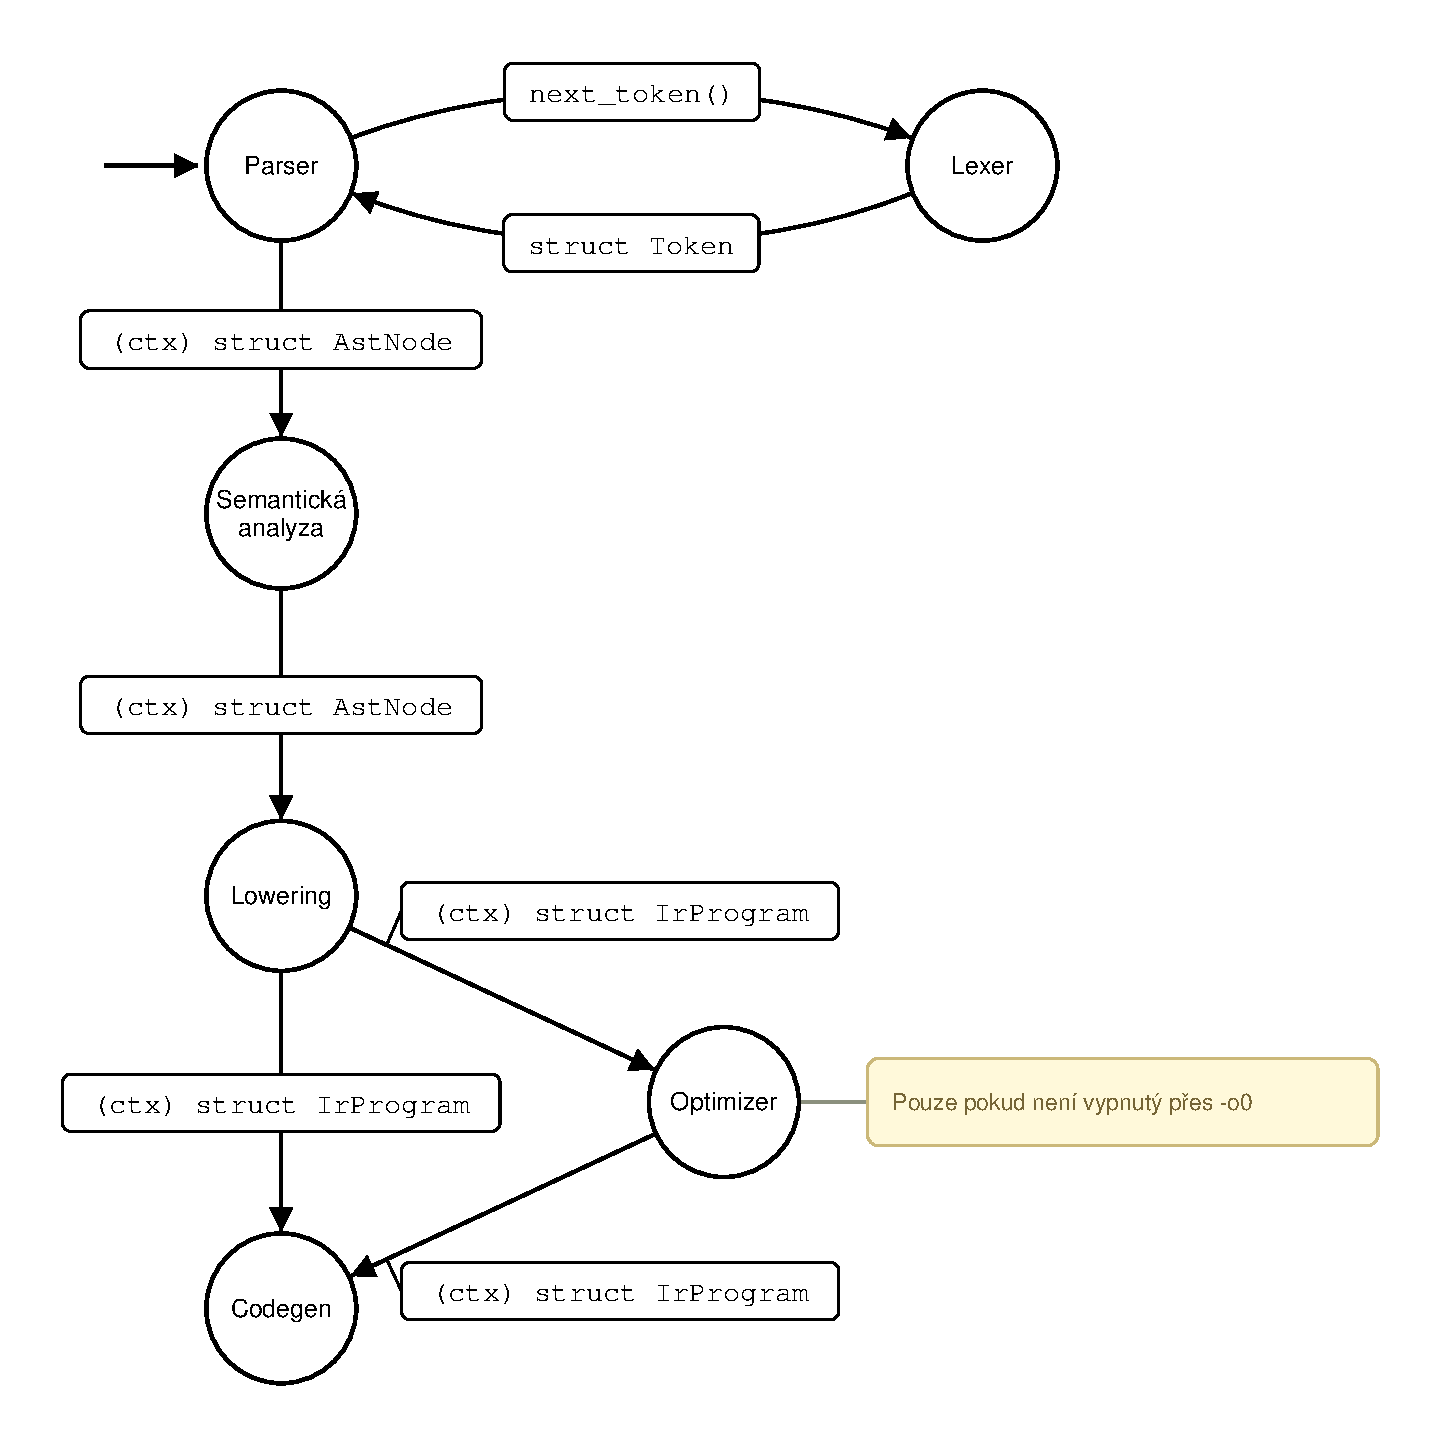
\includegraphics[width=\textwidth]{fig/schema.pdf}
  \caption{Blokové schéma architektury překladače}
  \label{fig:architektura}
\end{figure}

\TODO{textový popis komponent a datových toků (vstupy, výstupy, význam komponent a jejich propojení)}

% ============================================================================
% LEXIKÁLNÍ ANALÝZA
% Zadání: diagram automatu, který specifikuje lexikální analyzátor (podle
% konvencí přednášených v IFJ), s případným slovním popisem odchylek od
% standardního modelu konečného automatu.
% ============================================================================
\clearpage
\section{Lexikální analýza}

% #1 = stránka v lexer.pdf, #2 = popisek, #3 = odkaz
\newcommand{\lexerdiagram}[3]{
  \noindent\begin{minipage}[t]{\linewidth}
    \centering
    \makebox[\linewidth][c]{
      \includegraphics[page=#1,scale=.30,trim=23bp 23bp 23bp 23bp,clip]{fig/lexer.pdf}
    }
    \setlength{\abovecaptionskip}{4pt}
    \captionof{figure}{#2}
    \label{#3}
  \end{minipage}\par\smallskip
}

\TODO{případný slovní popis odchylek od standardního modelu konečného automatu}
Používáme deterministický zásobníkový automat, který má pouze mírné odchylky od standardního modelu.

Pro jednoduchost a velikost zápisu nejsou vypsána všechna pravidla pro zásobník, ale jsou sdružena čárkami (,).
Pokud je přechod možný pro všechny vrcholy zásobníku, značí ho \texttt{(any)}.

Přechody jsou umožněny pouze pokud je na levé straně od → stav na vrcholu zásobníku.
Máme definovaných několik operací:

\texttt{keep} je základní operace, která porovná vrchol zásobníku s vybraným stavem a nezmění zásobník.
Umožní přechod pouze v případě, že se vybraný stav shoduje s vrcholem.
Tato operace se provede v případě, že není v automatu specifikováno jinak (v přechodu není → ).

\texttt{push} je operace, která přidá nový prvek na vrchol zásobníku.

\texttt{pop} je operace, která odstraní prvek z vrcholu zásobníku.

\texttt{replace} je operace, která vrátí hodnotu vrcholu zásobníku.

\lexerdiagram{1}{Přehled konečného automatu lexikálního analyzátoru}
  {fig:automat}

\subsection{Skupiny stavů}
\lexerdiagram{2}{Numbers and Floats}
  {fig:lexer-numbers}

\lexerdiagram{3}{Division and Comments}
  {fig:lexer-comments}

\lexerdiagram{6}{Main}
  {fig:lexer-main}

\lexerdiagram{4}{Strings}
  {fig:lexer-strings}

\lexerdiagram{5}
  {Identifiers, S\_strings and Dollar expressions}
  {fig:lexer-identifiers}

\lexerdiagram{7}
  {triple\_S\_string string and end}
  {fig:lexer-triple-string}

\noindent
\begin{minipage}[t]{.48\linewidth}
  \lexerdiagram{8}
    {Less than and Control arrow}
    {fig:lexer-less-than}
\end{minipage}\hfill
\begin{minipage}[t]{.48\linewidth}
  \lexerdiagram{9}{Parenthesis and Unit}
    {fig:lexer-unit}
\end{minipage}

% ============================================================================
% SYNTAKTICKÁ ANALÝZA
% Zadání: LL gramatika a z ní vycházející LL tabulka; precedenční tabulka,
% podle které byl implementován syntaktický analyzátor výrazů.
% ============================================================================
\section{Syntaktická analýza}

\subsection{LL gramatika}
\TODO{LL gramatika}

\subsection{LL tabulka}

\begin{table}[htbp]
  \centering
  \caption{LL tabulka syntaktického analyzátoru}
  \label{tab:ll-tabulka}
  \TODO{LL tabulka}
\end{table}

\subsection{Precedenční tabulka}

\begin{table}[htbp]
  \centering
  \caption{Precedenční tabulka pro zpracování výrazů}
  \label{tab:precedencni-tabulka}
  \TODO{precedenční tabulka}
\end{table}

% ============================================================================
% POPIS MODULŮ
% Zadání: stručný popis každého modulu -- informačně obohacující věta
% na dvojici .c/.h. Identifikátary sázejte fontem s pevnou šířkou znaků.
% ============================================================================
\section{Popis modulů}

% Pro každý pár .c/.h přidejte jednu položku:
\begin{description}[style=nextline]
  \item[\ttfamily \TODO{soubor.c\,/\,soubor.h}] \TODO{stručný popis modulu}
  \item[\ttfamily \TODO{soubor.c\,/\,soubor.h}] \TODO{stručný popis modulu}
\end{description}

% ============================================================================
% POUŽITÉ ZDROJE
% Zadání: bibliografické citace všech převzatých zdrojů (vč. kódu
% a algoritmů).
% ============================================================================
\begin{thebibliography}{9}
  \bibitem{zdroj1} \TODO{bibliografická citace převzatého zdroje}
\end{thebibliography}

% ============================================================================
% VYUŽITÍ PROSTŘEDKŮ AI
% Zadání (sekce 4): uveďte konkrétní AI nástroje a modely a stručně popište
% typický pracovní postup při jejich použití; popište problémy, na které jste
% při využití AI narazili, a situace, ve kterých jste návrhy AI nevyužili
% nebo značně upravili.
% ============================================================================
\section{Využití prostředků AI}

\subsection{Použité nástroje a pracovní postup}
\TODO{konkrétní použité AI nástroje a modely + typický pracovní postup}

\subsection{Problémy a nevyužité návrhy}
\TODO{problémy při využití AI; situace, kdy návrhy nebyly využity nebo byly značně upraveny}

\end{document}
